\documentclass[14pt,a4paper]{scrartcl}
\usepackage[left=25mm, right=20mm, top=20mm, bottom=30mm]{geometry}
\usepackage[utf8]{inputenc}
\usepackage[english,russian]{babel}
\usepackage[T1]{fontenc}
\usepackage{times}
\usepackage{listings}
\usepackage[usenames,dvipsnames]{color}
\usepackage{enumitem}
\usepackage{graphicx}
\usepackage{tikz}
\usepackage{scrextend}
\usepackage{ragged2e}
\usepackage{microtype}
\usepackage{indentfirst}
\usepackage[toc,page]{appendix}

\justifying
\sloppy
\linespread{1,5}
\tolerance=500
\hyphenpenalty=10000
\emergencystretch=3em

\usetikzlibrary{trees,calc}
\usetikzlibrary{positioning}
\graphicspath{ {images/} }

\lstdefinelanguage{Dockerfile}{morekeywords={FROM, RUN, CMD, LABEL, MAINTAINER, EXPOSE, ENV, ADD, COPY, ENTRYPOINT, VOLUME, USER, WORKDIR, ARG, ONBUILD, STOPSIGNAL, HEALTHCHECK, SHELL}, morecomment=[l]{\#}, morestring=[b]"}

\lstset{language=R, basicstyle=\ttfamily, numbers=left, numberstyle=\color{Blue}, stepnumber=1, numbersep=5pt, backgroundcolor=\color{white}, showspaces=false, showstringspaces=false, showtabs=false, frame=single, rulecolor=\color{black}, tabsize=2, captionpos=b, breaklines=true, breakatwhitespace=false, keywordstyle=\color{RoyalBlue}, commentstyle=\color{YellowGreen}, stringstyle=\color{ForestGreen}}

\makeatletter
\newcount\dirtree@lvl
\newcount\dirtree@plvl
\newcount\dirtree@clvl
\def\dirtree@growth{%
  \ifnum\tikznumberofcurrentchild=1\relax
  \global\advance\dirtree@plvl by 1
  \expandafter\xdef\csname dirtree@p@\the\dirtree@plvl\endcsname{\the\dirtree@lvl}
  \fi
  \global\advance\dirtree@lvl by 1\relax
  \dirtree@clvl=\dirtree@lvl
  \advance\dirtree@clvl by -\csname dirtree@p@\the\dirtree@plvl\endcsname
  \pgf@xa=7mm\relax
  \pgf@ya=-13mm\relax
  \pgf@ya=\dirtree@clvl\pgf@ya
  \pgftransformshift{\pgfqpoint{\the\pgf@xa}{\the\pgf@ya}}%
  \ifnum\tikznumberofcurrentchild=\tikznumberofchildren
  \global\advance\dirtree@plvl by -1
  \fi
}

\tikzset{
  dirtree/.style={
    growth function=\dirtree@growth,
    every node/.style={anchor=north},
    every child node/.style={anchor=west},
    edge from parent path={(\tikzparentnode\tikzparentanchor) |- (\tikzchildnode\tikzchildanchor)}
  }
}
\makeatother

\begin{document}

    % Титульник
    \begin{titlepage}
        \begin{center}
            \large
            МИНИСТЕРСТВО ОБРАЗОВАНИЯ И НАУКИ\\
            РОССИЙСКОЙ ФЕДЕРАЦИИ\\
            \textbf{Федеральное агентство по образованию\\}
            \vspace{0.5cm}
            ТВЕРСКОЙ ГОСУДАРСТВЕННЫЙ УНИВЕРСИТЕТ\\
            \vspace{0.25cm}
            Факультет прикладной математики и информатики\\
            Кафедра математической статистики и системного анализа\\
            \vfill
            \textsc{ВЫПУСКНАЯ РАБОТА БАКАЛАВРА}\\[5mm]
            {\LARGE Разработка модуля непараметрического анализа данных в пакете R\\[2mm]}
            \bigskip
        \end{center}
        \vfill
        \hfill
        \begin{minipage}{0.4\textwidth}
			Допущен к защите:\\
			<<\rule{0.12\textwidth}{0.4pt}>>\rule{0.45\textwidth}{0.4pt}2018г.\\
			{\bf Руководитель ООП:}\\

			\rule{0.50\textwidth}{0.4pt}{/А.В. Язенин/}\\
			{ \bfЗаведующий кафедрой:} {математической статистики и системного анализа}\\

			\rule{0.50\textwidth}{0.4pt}{/В.Н. Михно/}
		\end{minipage}
		\hfill
		\begin{minipage}{0.4\textwidth}
			\begin{flushleft}
		        Автор:\\
		        Семенков Филипп Андреевич\\

		        Научный руководитель:\\
		        Сидорова Оксана Игоревна\\
			\end{flushleft}
        \end{minipage}
        \vfill
        \begin{center}
            Тверь, 2018 г.
        \end{center}
    \end{titlepage}

    % Оглавление
    \newpage
    \tableofcontents

    % Содержание
    % Теория
    \newpage
    \section{Теоретическая часть}
    \subsection{Введение}
    В учебном плане факультета прикладной математики и кибернетики на кафедре математической статистики и системного анализа мы изучаем довольно большое количество различных дисциплин. В курсе непараметрической статистики мы изучаем нормальное и экспоненциальное распределения, гамма --- распределения, логарифмически нормальные и другие. Для решения задач непараметрической статистики используются методы, позволяющие изучать выборку небольшого объема с данными в которых содержатся такие параметры, о распределении которых мало известно или абсолютно ничего не известно. Такие методы не основаны на оценке параметров.

    \subsection{Предмет и задачи непараметрической статистики}
    Математическая статистика --- это наука о математических методах, позволяющих по статистическим данным построить теоретико–вероятностную модель исследуемого явления. Математическая статистика имеет тот же предмет, что и теория  вероятностей --- изучение случайных экспериментов с неопределенным исходом, в которых выполнено свойство устойчивости частот, но решает задачи, в некотором  смысле обратные, к задачам теории вероятностей.

    Основная задача состоит в том, чтобы на основе экспериментальных данных (наблюдений) сузить класс $P$ априорно заданных вероятностных мер до некоторого более узкого подкласса $P0 \subset P$ (в идеале выбрать одно распределение).

    В математической статистике существуют два основных подхода к решению этой задачи ---  параметрический и непараметрический. Эти подходы обусловили возникновение двух больших групп методов, дополняющих друг друга, но, вместе с тем, противостоящих и конкурирующих.

    Параметрические методы основаны на предпосылке о том, что статистические данные имеют закон распределения, принадлежащий к тому или иному параметрическому семейству P --- нормальному, показательному и т.п.

    Непараметрические критерии (критерии значимости, не зависящие от распределения) не требуют предварительных предположений относительно вида исходного распределения и используют лишь минимальную априорную информацию о фундаментальных свойствах случайных величин (непрерывность, симметрия функции распределения и т.п.) и могут использоваться в тех случаях, когда применение параметрических статистических методов либо сомнительно, либо неуместно, например, при обработке данных, не обладающих количественной природой.

    \subsection{Что такое R?}
	R --- система статистических вычислений и графики. Он состоит из языка и среды выполнения с графикой, отладчик, доступ к определенным системным функциям и возможность запуска программ, хранящихся в файлах сценариев.

	R --- язык широко используется среди статистиков и сбора данных для разработки статистического программного обеспечения и анализа данных. Опросы и обзоры показывают, что популярность R значительно увеличилась в последние годы.

	R --- реализация языка программирования S в сочетании с семантикой лексической семантики, вдохновленной Схемой. S был создан Джоном Чемберсом в Bell Labs. R был создан Росом Ихакой и Робертом Джентльменом в Университете Окленда, Новая Зеландия, и в настоящее время разрабатывается группой разработчиков R Development Core, членом которой является Чемберс. R называется частично после первых имен первых двух авторов R и частично как игра на имя S.

	R --- проект GNU. Исходный код для программной среды R написан в основном в C, Fortran и R. R свободно доступен в соответствии с GNU General Public License, а предварительно скомпилированные двоичные версии предоставляются для различных операционных систем. R использует интерфейс командной строки; однако несколько графических пользовательских интерфейсов доступны для использования с R \cite{R-wiki}.

    \subsection{Практическая ценность}
    Для решения таких задач используются различные статистические пакеты, такие как пакет R. В пакете R существует большое количество библиотек, содержащих готовые функции, которые помогут решить задачу.

    Для вызова подобных функций, необходимо проделать несколько шагов:

    \begin{itemize}[noitemsep]
        \item Установка пакета R
        \item Поиск библиотеки с необходимой функцией
        \item Установка библиотеки
        \item Написание программы для вызова функции
    \end{itemize}

    Установить сам интерпретатор R довольно просто. К тому же для этого языка существуют IDE. Самый популярный из них это RStudio. RStudio в общем упрощает написание программы на языке R. Он включает в себя редактор кода, инструменты для отладки и визуализации. Найти и установить необходимую библиотеку не так просто. Необходимые функции разбросаны по разным пакетам. А некоторые пакеты имеют специфические зависимости, на установку и настройку которых может потребоваться много времени. Да и для написания программы необходимы знания языка и время на изучение пакетов. Всё это натолкнуло меня на мысль о создании универсального модуля в котором будут собраны необходимые пакеты.

    \subsection[Задел на будущее]{Задел на будущее}
    Просто собрать необходимые пакеты в одну программу это сложная задача, но ещё сложнее предоставить к нужным функциям единый удобный интерфейс, который можно будет использовать на различных устройствах. Для того, чтобы в любой момент можно было добавить или удалить функцию, поменять её описание и при этом не сломать всё остальное стоит разработать программный интерфейс приложения (API). API может помочь в наполнении программы функциями, а так же позволит использовать модуль не только в решении задач непараметрической статистики. В таком случае этот модуль будет полезен не только в рамках поставленной задачи.

    \subsection{Постановка задачи}
    \noindent Цель: Разработать модуль непараметрического анализа данных в пакете R.
	\noindent Задачи:
    \begin{enumerate}
        \item Разработать требования к программе
        \item Выбрать и изучить стек технологий, согласно требованиям
        \item Разработать структуру приложения
        \item Написать приложение
    \end{enumerate}

    \subsection{Требования к программе}
    Требования к поведению программы:
    \begin{itemize}
        \item Модуль должен являться приложением, написанным на языке R
        \item Модуль должен позволять решать задачи непараметрической статистики
        \item Модуль должен иметь пользовательский интерфейс
    \end{itemize}

    Требования к характеру поведения системы:
    \begin{itemize}
        \item Модуль должен иметь возможность расширения функционала
        \item Доступ к модулю может осуществляться с помощью различных устройств
        \item Устройства могут иметь различные операционные системы
        \item Пользовательский интерфейс должен корректно отображаться на устройствах с различными экранами
    \end{itemize}

    \subsection{Пользовательский интерфейс}
    Согласно требованиям к поведению программы, модуль должен иметь пользовательский интерфейс. Существует несколько видов пользовательских интерфесов.

    Основные виды пользовательских интерфесов:
    \begin{itemize}
        \item Консольный интерфейс
        \item Графический:
        \begin{itemize}
            \item Простой графический интерфейс
            \item WEB интерфейс
        \end{itemize}
    \end{itemize}

    Так как модуль должен являться приложением, написанным на языке R, то можно сделать ограничение написания интерфейса на языке R, чтобы не усложнять модуль различными языками программирования. Можно понять, что интерфейс должен отобразить решения задач непараметрической статистики. В таком случае следует учесть, что результатом может быть график. Также согласно требованиям к характеру поведения системы стоит учесть, что интерфейс должен корректно отображаться на различных устройствах с различными оперционными системами.

    Для того, чтобы определиться с видом пользовательского интерфейса, необходимо понять, какой из них лучше всго соответствует требованиям. При выборе консольного интерфейса могут возникнуть проблемы при отображении графиков, в таком случае нам больше подойдёт один из графических интерфейсов. Если мы выберем простое графическое (оконное) приложение, то в силу различных операционных систем могут возникнуть проблемы с переносом приложения. К тому же, по данным агентства 'We Are Social', возросло количество интернет-пользователей, большинство из них являются владельцами смартфонов \cite{Internet-statistic-2018}. Из этого всего следует, что приложение должно предоставлять web интерфейс.

    \subsection[Программный интерфейс приложения]{Программный интерфейс приложения (API)}
    Программный интерфейс приложения должен предоставлять возможность внедрить необходимую функцию в модуль. Стоит определить как в конечном итоге будет выглядеть функция и какой программный интерфейс необходимо предоставить. С точки зрения программирования, функция --- это подпрограмма, которая принимает параметры и возвращает некоторый результат. С точки зрения математики, функция --- это алгоритм, который также принимает параметры и возвращает некоторый результат. Для того чтобы в модуле различать функции, необходимо им выдать уникальные идентификаторы (названия функций). Чтобы лучше понимать что делает алгоритм стоит добавить описание.

    В конечном итоге становится понятным, интерфейс будет ожидать от наших подпрограмм:
    \begin{itemize}
        \item Название функции
        \item Описание функции
        \item Алгоритм
        \item Типы, имена и значения входных данных
        \item Типы, имена и значения выходных данных
    \end{itemize}
    На выходе API должен собрать такие подпрограммы и предоставить пользовательский интерфейс.

    \subsection[Развёртывание приложения]{Развёртывание приложения}
    Веб-приложение — это приложение, логика которого распределена между клиентом и сервером (клиент-серверное приложение) \cite{Web-app-wiki}. Клиентская часть веб-приложения представляет собой графический интерфейс. Это то, что пользователь видит на странице. Этот интерфейс отображается в браузере. Пользователь в свою очередь взаимодействует с веб-приложением через браузер. Сервером называется компьютер, выделенный из группы персональных компьютеров для выполнения какой-либо задачи без непосредственного участия человека \cite{Server}. Выделяют также веб сервер. Это сервер содержащий программу или скрипт, который обрабатывает запросы пользователя (точнее, запросы браузера) \cite{Web-app-struct}

    Выбор технологии для разворачивания веб приложения на сервере будут рассмотрены в практической части.

    % Практика
    \newpage
    \section[Практическая часть]{Практическая часть}
    \subsection[Выбор технологий]{Выбор технологий}
    В рамках задачи, необходимо определить, с помощью каких инструментов будет:
    \begin{itemize}
        \item разворачиваться сервер
        \item обрабатываться html запросы
        \item генерироваться пользовательский интерфейс
    \end{itemize}

    Для того чтобы развернуть приложение существует несколько возможных решений.

    Решение "в лоб" это написание установочного скрипта, который установит всё, что необходимо и запустит приложение на сервере (скрипт может быть как простым bash (sh) скриптом, так и чем-то сложным, созданным с использованием специальных инструментов). Недостатки такого подхода — это неустойчивость к ошибкам и плохая переносимость. Насколько бы хорошо не был написан скрипт, он не сможет учесть все возможные варианты развития событий., что скорее всего приведёт к остановке исполнения скрипта с ошибкой. Но при этом, скрипт уже мог внести какие-либо изменения, которые сложно или невозможно 'откатить'.

    Чтобы не было таких проблем можно запустить приложение в облачном сервисе. На виртуальный сервер вручную установить всё что нужно. У такого подхода есть недостатки. Виртуальные сервера довольно медленны, мы не можем быть уверены в их безопсности и стабильности.

    Из этого следует, что веб приложение стоит запускать на своём сервере, но при этом необходимо каким-то образом ограничить влияние нашего приложения (установка пакетов, занимание портов, изменения системных файлов и прочее) от других приложений, которые будут или уже запущены на сервере. На помощь приходят виртуальные машины. На сервере можно выделить часть ресурсов сервера для запуска виртуальной машины с нужной операционной системой и необходимым окружением. Этот вариант неплох, но имеет свои недостатки. Виртуальные машиные ресурсоёмкие и громозкие.

    Для решения всех этих недостатков можно использовать Docker. Как и в виртуальной машине, в докере запускается заранее настроенная операционная система в которой и запускается приложение. Но при этом не запускается отдельная виртуальная машина, которой выделяются ресурсы. Все процессоры и память делится докером между всем запущенными приложениями в системе. Такой подход можно расположить между запуском приложения на самом сервере и на виртуальной машине. В конечном итоге получается, что приложение запустится в собственном окружении, но при этом будет полный доступ к ресурсам. Любые изменения в этом окружении никак не повлияют на всё остальное. Подход, используемый докером называется контейнеризацией.
    \newline
    \newline
    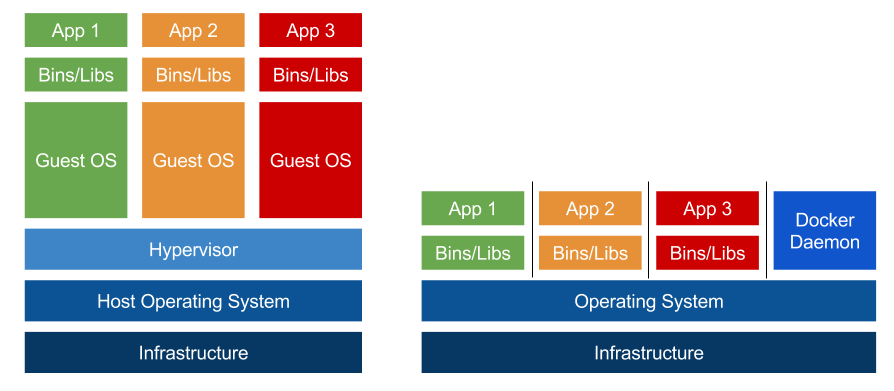
\includegraphics[width=\textwidth]{Docker-struct.png}
    \newpage
    Для создания пользовательского интерфейса я выбрал пакет shiny. Shiny --- это фреймворк для разработки веб приложений написанный для пакета R. Он позволяет легко создавать и запускать интерактивные веб-приложения. Этот фреймворк в свою очередь использует Bootstrap. Bootstrap — это свободный набор инструментов для создания сайтов и веб-приложений. Он включает в себя HTML- и CSS-шаблоны оформления для типографики, веб-форм, кнопок, меток, блоков навигации и прочих компонентов веб-интерфейса, включая JavaScript-расширения. Простейший проект, с использованием shiny, должен иметь две функции – ui (описание ввода-вывода) и server (все вычисления).

    \subsection[Развёртывание приложения]{Развёртывание приложения}

    Для того чтобы развернуть приложение необходимо написать dockerfile. В нем необходимо указать какая ОС необходима, на каком порту будет запущено приложения и как его запустить. Чаще всего есть некоторый похожий сценарий для установки и настройки ОС, поэтому такие инструкции чаще всего уже написаны и выложены в dockerHub. Такие инструкции можно подключать, чтобы не писать одинаковый код.

    За основу возьмём r-base.
    \begin{lstlisting}[language=Dockerfile]
FROM r-base
    \end{lstlisting}
    После этой команды будет установлен debian и будет установлен интерпретатор R. После чего скопируем данные нашего приложения.
    \begin{lstlisting}[language=Dockerfile]
RUN mkdir npsw
COPY . npsw
WORKDIR npsw
    \end{lstlisting}
    Укажем порт для прослушивания соединения в контейнере.
    \begin{lstlisting}[language=Dockerfile]
EXPOSE 3838
    \end{lstlisting}
    И запустим приложение.
    \begin{lstlisting}[language=Dockerfile]
CMD ["./npsw"]
    \end{lstlisting}

    \subsection[Алгоритм запуска приложения]{Алгоритм запуска приложения}
    Укажем путь до интерпретатора R.
    \begin{lstlisting}[language=R]
#!/usr/bin/Rscript
    \end{lstlisting}

    Устновим зависимости если это необходимо.
    \begin{lstlisting}[language=R]
if(!require(shiny)){install.packages("shiny")}
if(!require(npsm)){install.packages("npsm")}
if(!require(Rfit)){install.packages("Rfit")}
    \end{lstlisting}

    Подключим пакеты R.
    \begin{lstlisting}[language=R]
library(shiny)
library(npsm)
library(Rfit)
    \end{lstlisting}

    Укажем путь до исходного кода и порт
    \begin{lstlisting}[language=R]
appDir = "src"
port = 3838
    \end{lstlisting}

    Запустим приложение
    \begin{lstlisting}[language=R]
runApp(appDir = appDir, port = port)
    \end{lstlisting}

    \subsection[Программный интерфейс приложения]{Программный интерфейс приложения (API)}
    Наш API будет искать модули с функциями в папке "modules".
    \begin{lstlisting}[language=R]
MODULES_PATH = "modules"
    \end{lstlisting}
    Для перечисления всех файлов в этой папке используем команду
    \begin{lstlisting}[language=R]
MODULES = list.dirs(
    path = MODULES_PATH,
    full.names = FALSE,
    recursive = FALSE
)
    \end{lstlisting}
    Если неободимо использовать только конкретные модули в конкретном порядке то прописываем вручную.
    \begin{lstlisting}[language=R]
MODULES = c( '', '' ... )
    \end{lstlisting}
    Так как shiny ожидает описание страницы в виде двух функций (server и ui) то пусть наши функции будут предоставлять 2 файла с такими именами
    \begin{lstlisting}[language=R]
UI_FILENAME = "ui.R"
SERVER_FILENAME = "server.R"
    \end{lstlisting}

    \subsubsection[Пользовательский интерфейс]{Пользовательский интерфейс}
    Опишем основной файл с описанием shinyApp. Назовём нашу программу 'NPSW' (Nonparametric Statistical Methods Web) и установим навигационную панель (для выбора модуля) с именем нашего приложения.
    \begin{lstlisting}[language=R]
PROGRAM_TITLE = 'NPSW'

shinyApp(
    do.call(
        navbarPage, c(
            title = PROGRAM_TITLE,
            ...
    \end{lstlisting}
    Теперь необходимо пройтись по модулям, добавить вкладки и узнать какие функции в модулях есть.
    \begin{lstlisting}[language=R]
lapply(
    1 : length(MODULES),
    function(i) {
        FUNCTIONS = list.dirs(
            path = paste(
                MODULES_PATH,
                MODULES[i],
                sep="/"
            ),
            full.names = FALSE,
            recursive = FALSE
        )
        tabPanel(
            MODULES[i],
            ...
    \end{lstlisting}
    В конечном итоге осталось для каждой функции отрисовать UI который описан в файле описания интерфейса для конкретной функции.
    \begin{lstlisting}[language=R]
lapply(
    1 : length(FUNCTIONS),
    function(j) {
        dget(
            paste(
                MODULES_PATH,
                MODULES[i],
                FUNCTIONS[j],
                UI_FILENAME,
                sep = "/"
            )
        )
    }
)
    \end{lstlisting}

    \subsubsection[Вычисления]{Вычисления}
    Все вычисления происходят в отдельной функции, которая принимает три параметра.
    \begin{lstlisting}[language=R]
function(input, output, session)
    \end{lstlisting}
    Где:
    \begin{itemize}
        \item \textbf{input}  --- данные которые ввёл пользователь
        \item \textbf{output} --- данные которые вернул сервер
        \item \textbf{session} --- сессия пользователя
    \end{itemize}

    Также как и с интерфейсом, пробежимся по модулям
    \begin{lstlisting}[language=R]
lapply(
    1 : length(MODULES),
    function(i) {
        FUNCTIONS = list.dirs(
            path = paste(
                MODULES_PATH,
                MODULES[i],
                sep="/"
            ),
            full.names = FALSE,
            recursive = FALSE
        )
        ...
    \end{lstlisting}
    После чего пробежимся по функциям и получим алгоритмы которые описаны в файле server.R
    \begin{lstlisting}[language=R]
lapply(
    1 : length(FUNCTIONS),
    function(j) {
        func <- dget(
            paste(
                MODULES_PATH,
                MODULES[i],
                FUNCTIONS[j],
                SERVER_FILENAME,
                sep = "/"
            )
        )
        func(input, output, session)
    }
)
    \end{lstlisting}

    \newpage
    \subsection[Cтруктура приложения]{Cтруктура приложения}
    В конечном итоге получаем следующую струтуру приложения:\\
	\newline
	\begin{tikzpicture}[dirtree]
        \node {npsw/}
            child { node {src/}
                child { node {modules}
                    child { node {module1/}
                        child { node {server1.R} }
                        child { node {ui1.R} }
                    }
                    child { node {module2/}
                        child { node {server2.R} }
                        child { node {ui2.R} }
                    }
                    child { node {.....} }
                }
                child { node {util}
                    child { node {utilFunction1.R} }
                    child { node {utilFunction2.R} }
                    child { node {.....} }
                }
                child { node {app.R} }
            }
            child { node {npsw} }
            child { node {Dockerfile} };
	\end{tikzpicture}
    \newline
    Где:
    \begin{itemize}
        \item \textbf{npsw/}  --- директория приложения
        \item \textbf{npsw} --- скрипт, запускающий приложение
        \item \textbf{Dockerfile} --- скрипт, разворачивающий сервер
        \item \textbf{src/} --- директория исходного кода приложения
        \item \textbf{app.R} --- код, описывающий API
        \item \textbf{modules/} --- директория, содержащая модули, соответствующие написанному API
        \item \textbf{module1/} --- директория одного из модулей
        \item \textbf{server1.R} --- файл, описывающий алгоритм модуля 'module1'
        \item \textbf{ui1.R} --- функция, описывающая пользовательский интерфейс модуля 'module1'
        \item \textbf{util/} --- директория, содержащая утилитарные функции
        \item \textbf{utilFunction1.R} --- файл, описывающий утилитарную функцию
    \end{itemize}

    % Примеры
    \newpage
    \section[Примеры решения задач]{Примеры решения задач}
    \subsection[Анализ дихотомических данных]{Анализ дихотомических данных}
    Исследовалась проблема условного досрочного освобождения уголовников. Для этого изучалось поведение всех уголовников --- мужчин, впервые условно освобожденных под специальный надзор из тюрем Нью --- Йорка в 1958 --- 1959 гг.

	Все освобожденные находились под наблюдением 3 года после освобождения, если какое --- либо правонарушение не прекращало действие освобождения раньше.

	В этом исследовании, где фигурировало очень много осужденных, Стэнтон рассматривал преступников, признанных виновными в иных преступлениях, чем убийство. Он обнаружил, что около 60\% всех освобожденных не совершают каких --- либо правонарушений в течение трех лет после освобождения.

	Стэнтон обнаружил также, что в течение тех же трех лет 56 из 65 освобожденных досрочно на поруки убийц также не совершали каких --- либо правонарушений, приостанавливающих условное освобождение.

	Будем считать, что отсутствие правонарушений у мужчин --- убийц, находящихся в течение трех лет под надзором --- это «успех» в испытаниях Бернулли.

	Задание: Обозначим B --- число успехов = отсутствие правонарушений у мужчин --- убийц в n независимых испытаниях по схеме Бернулли. Пусть в 10 испытаниях «успех» появился 7 раз (искусственный пример). Используя биномиальный критерий, осуществите проверку гипотезы H0 : p = 0.6, против альтернатив H1 : p > 0.6, H1 : p < 0.6 и H1 : p $\ne$ 0.6

	Такую задачу можно решить с помощью языка R.

	Пусть задано $\alpha$ = 0.05, n = 10, p = 0.6. Соответствующие квантили биномиального закона находим по правилу:
    \begin{itemize}
        \item \textbf{нижняя}: qbinom(0.05, 10, 0.6, lower.tail = TRUE, log.p = FALSE)
        \item \textbf{верхняя}: qbinom(0.95, 10, 0.6, lower.tail = TRUE, log.p = FALSE)
    \end{itemize}

	Реально достигнутые уровни (у дискретного распределения могут отличаться от заявленного $\alpha$):
    \begin{itemize}
        \item \textbf{квантили}: q <- c(0, 1, 2, 3, 4, 5, 6, 7, 8, 9, 10)
        \item \textbf{нижняя}: 1-pbinom(q, 10, 0.6, lower.tail = TRUE, log.p = FALSE)
        \item \textbf{верхняя}: pbinom(q, 10, 0.6, lower.tail = TRUE, log.p = FALSE)
    \end{itemize}

	С помошью пеализованного API добавим функцию qbinom

    server.R
    \begin{lstlisting}[language=R]
function(input, output, session) {
    output$qbinomResult <- renderPrint({
        qbinom(
            stringToArray(input$qbinomP),
            input$qbinomSize,
            input$qbinomProb,
            lower.tail = input$qbinomLowerTail,
            log.p = input$qbinomLogP
            )
    })
}
    \end{lstlisting}

    ui.R
    \begin{lstlisting}[language=R]
sidebarLayout(
    sidebarPanel(
        textInput(
            "qbinomP",
            "vector of quantiles"
        ),
        numericInput(
            "qbinomSize",
            label="number of observations"
        ),
        sliderInput(
            "qbinomProb",
            label="probability of success on each trial",
            min = 0,
            max = 1
        ),
        checkboxInput(
            "qbinomLowerTail",
            label="probabilities are F(x) = P(X <= x), otherwise P(X > x) = 1 --- F(x)."
        ),
        checkboxInput(
            "qbinomLogP",
            label="probabilities p are given as log(p)"
        )
    ),
    mainPanel(
        h2("qbinom()"),
        h3("Density, distribution function, quantile function and random generation for the binomial distribution with parameters size and prob"),
        h5("Syntax: qbinom(p, size, prob, lower.tail = TRUE, log.p = FALSE)."),
        verbatimTextOutput("qbinomResult")
    )
)
    \end{lstlisting}

    \newpage
    После чего запустим приложение и введём данные. Получим следующий результат:\\

    qbinom(0.05, 10, 0.6, lower.tail = TRUE, log.p = FALSE)\\
    
    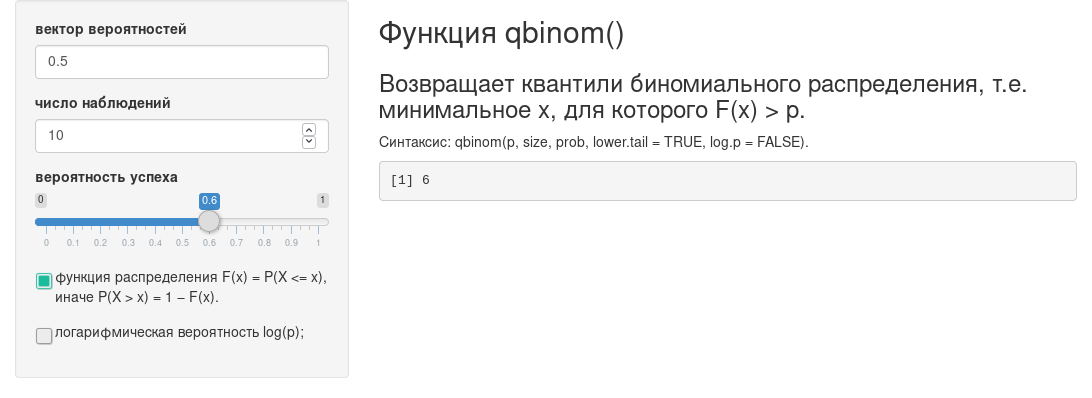
\includegraphics[width=\textwidth]{qbinom.png}

    qbinom(0.95, 10, 0.6, lower.tail = TRUE, log.p = FALSE)\\

    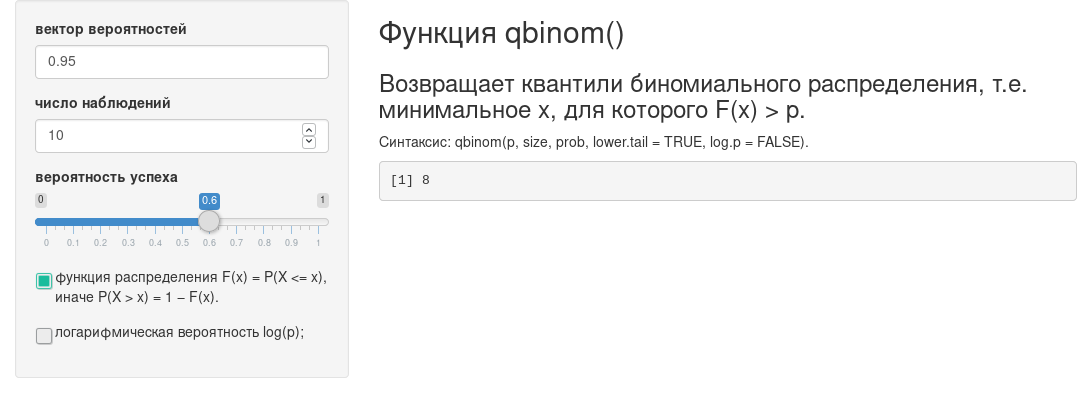
\includegraphics[width=\textwidth]{qbinom-2.png}

    \newpage
    По аналогии реализуем функцию pbinom. Получим следующий результат:\\

    pbinom(q, 10, 0.6, lower.tail = TRUE, log.p = FALSE)\\

    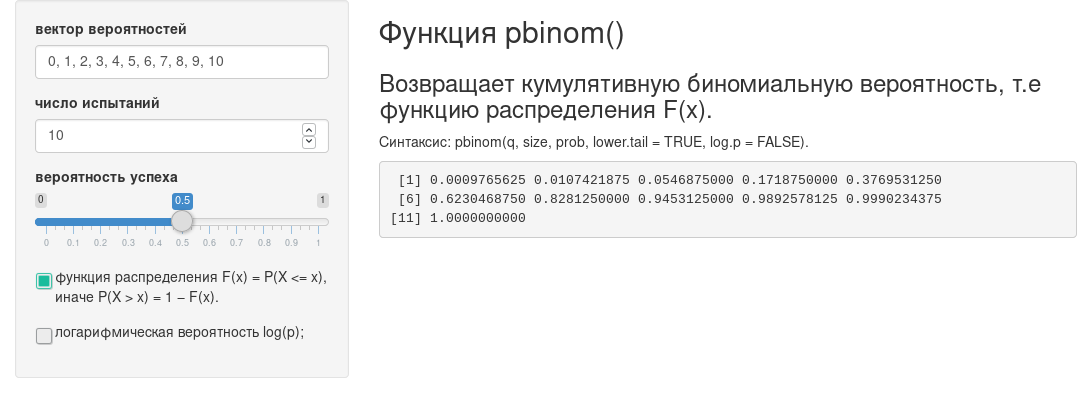
\includegraphics[width=\textwidth]{pbinom-1.png}

    \subsection{Тесты на сдвиги}

     Необходимо выяснить, отличается ли потребление энергии в группе обследованных женщин от рекомендованного значения 7725 кДж/сутки. Для выполнения теста Уилкоксона в системе R используется функция wilcox.test():
    Данные о суточном потреблении энергии (кДж/сутки) у 11 женщин. \cite{Altman} \\
    5260, 5470, 5640, 6180, 6390, 6515, 6805, 7515, 7515, 8230, 8770

	С помошью реализованного API добавим функцию wilcox.test

    server.R
    \begin{lstlisting}[language=R]
function(input, output, session) {
    output$wilcoxTestResult <- renderPrint({
        wilcox.test(
            x = stringToArray(input$wilcoxTestX),
            y = stringToArray(input$wilcoxTestY),
            alternative = input$wilcoxTestAlternative,
            mu = input$wilcoxTestMu,
            paired = input$wilcoxTestPaired,
            correct = input$wilcoxTestCorrect,
            conf.int = input$wilcoxTestConfInt,
            conf.level = input$wilcoxTestConfLevel
        )
    })
}
    \end{lstlisting}

    После чего запустим приложение и введём данные. Получим следующий результат:\\
    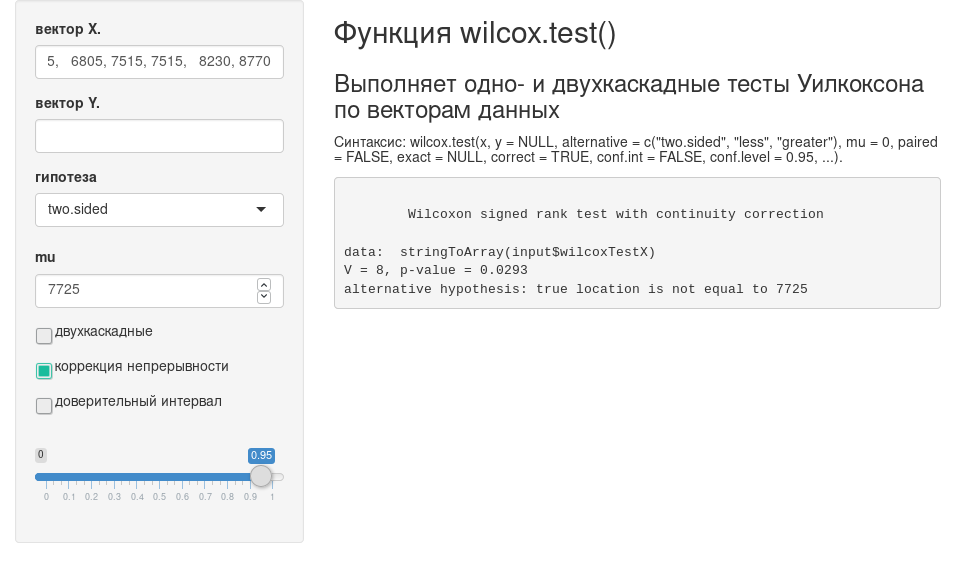
\includegraphics[width=\textwidth]{wilcox.png}
    Видим, что рассчитанное значение критерия V = 8. Вероятность получить такое (или превышающее его) значение при условии, что нулевая гипотеза верна, не превышает 0.05 (p-value = 0.0293). Это позволяет нам отклонить нулевую гипотезу о том, что суточное потребление энергии у обследованных 11 женщин не отличается от принятой нормы. Обратите внимание на выданное программой предупреждение о том, что полученное значени вероятности Р не является точным из-за наличия в данных повторяющихся значений (Warning message... cannot compute exact p-value with ties).

    \subsection{Тесты на равенство дисперсий}
    Проводится оценка прочности парашютов в зависимости от поставщика синтетических волокон.\\
    Данные измерений первого поставщика: 18.5, 24, 17.2, 19.4\\
    Данные измерений второго поставщика: 26.3, 25.3, 24, 24.2\\
    Проверим однородность обработок с помощью критерия Краскела–Уоллиса. Нулевая гипотеза, которую мы проверим при помощи теста Краскела-Уоллиса, заключается в том, что качество исследованных парашютов не зависит от произодителя.\\
    С помошью реализованного API добавим функцию kruskal.test, после чего запустим приложение и введём данные. Получим следующий результат:\\

    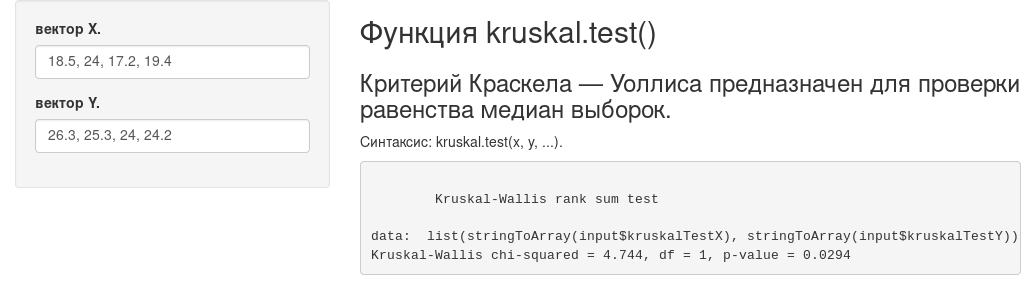
\includegraphics[width=\textwidth]{kruskal.png}

    Как видно из полученного результата, вероятность получить столь высокое наблюдаемое значение Н-критерия при верной нулевой гипотезе крайней мала и, следовательно, мы можем смело эту гипотезу отклонить.

%    \subsection{Непараметрическая корреляция}
%    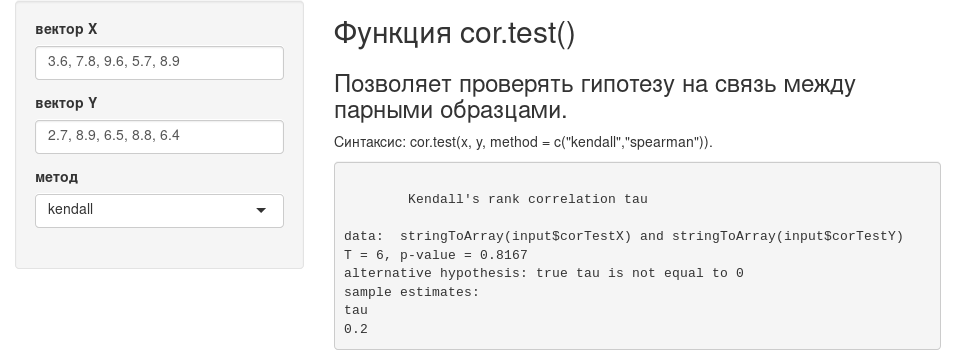
\includegraphics[width=\textwidth]{cor.png}
%    \subsection{Тесты на независимость}
%    \subsection{Распределения}


%X: "18.5, 24, 17.2, 19.4, 26.3, 25.3, 24, 24.2"
%Y: "20.6, 25.2, 20.8, 24.7, 24.5, 19.5, 22.6, 17.5"


    % Заключение
    \newpage
    \section[Заключение]{Заключение}

    В ходе решения задачи:
    \begin{itemize}
        \item изучны различные пакеты, позволяющие произвести непараметрический анализ данных.
        \item изучны паттерны проектирования приложения.
        \item изучен фреймворк shiny, позволяющий создавать web приложения в пакете R.
        \item изучен инструмент для разворачивания приложния --- docker.
        \item разработан пользовательский интерфейс приложения
        \item разработан API для внедрения / редактирования функций непараметрического анализа
        \item разработан dockerfile для разворачивания приложения
        \item произведено тестирование приложения
    \end{itemize}

    Были внедрены следующие модули и функции непараметрического анализа данных:

    \begin{center}
        \begin{tabular}{ccc}
            \textbf{Анализ дихотомических данных} & binom.test, prop.test\\
            \textbf{Тесты на сдвиги} & wilcox.test, mood.test\\
            \textbf{Тесты на равенство дисперсий} & kruskal.test\\
            \textbf{Непараметрическая корреляция} & cor, cor.test\\
            \textbf{Тесты на независимость} & mcnemar.test\\
            \textbf{Распределения} & pbinom, pnorm, qbinom, qchisq, qnorm\\
        \end{tabular}
    \end{center}

    В конечном итоге был разработан модуль непараметрического анализа данных в пакете R.

    % Список литературы
    \newpage
    \addcontentsline{toc}{section}{Список литературы}
    \begin{thebibliography}{9}
        \bibitem{R-wiki}R (язык программирования)
        \newblock --- https://ru.wikipedia.org/wiki/R

        \bibitem{Internet-statistic-2018}Social media use jumps in Q1 despite privacy fears
        \newblock --- https://wearesocial.com/uk/blog/2018/04/social-media-use-jumps-in-q1-despite-privacy-fears

        \bibitem{Web-app-wiki}Веб-приложение
        \newblock --- https://ru.wikipedia.org/wiki/Веб-приложение

        \bibitem{Server}Сервер (аппаратное обеспечение)
        \newblock --- https://ru.wikipedia.org/wiki/Сервер

        \bibitem{Web-app-struct}Структура веб-приложения
        \newblock --- http://labaka.ru/likbez/struktura-veb-prilozheniya

        \bibitem{Docker-habra}Docker. Зачем и как
        \newblock --- https://habr.com/post/309556

        \bibitem{Bootstrap-wiki}Bootstrap
        \newblock --- https://ru.wikipedia.org/wiki/Bootstrap

        \bibitem{Altman}Practical Statistics for Medical Research, Chapman Hall, London
        \newblock --- Altman D. G. (1981)

    \end{thebibliography}

\end{document}
